\section{锁的原理}
\subsection{LockSupport}

LockSupport 是个工具类,没有公有的构造函数。它的主要作用是挂起和唤醒线程,是创建锁和其他同步类的基础:

\begin{Java}
public class LockSupport {
    private static final Unsafe U = Unsafe.getUnsafe();
}
\end{Java}

LockSupport类与每个使用它的线程都会关联一个许可证,在默认情况下调用 LockSupport 类的方法的线程是不持有许可证的。

\subsubsection*{park() 方法}

park 系方法是 LockSupport 的核心方法,本质上是调用 Unsafe 的 park() 方法,具体方法实现是不可知的:

\begin{Java}
public static void park() {
    U.park(false, 0L);
}
\end{Java}

如果调用park方法的线程已经拿到了与LockSupport关联的许可证,则调用LockSupport.park()时会马上返回,否则调用线程会被禁止参与线程的调度,也就是会被阻塞挂起。

在其他线程调用 unpark(Thread thread)方法并且将当前线程作为参数时,调用park方法而被阻塞的线程会返回。另外,如果其他线程调用了阻塞线程的interrupt()方法,设置了中断标志或者线程被虚假唤醒,则阻塞线程也会返回。所以在调用park方法时最好也使用循环条件判断方式。

需要注意的是,因调用park()方法而被阻塞的线程被其他线程中断而返回时并不会抛出InterruptedException异常。

\subsubsection*{unpark(Thread thread) 方法}

\begin{Java}
public static void unpark(Thread thread) {
    if (thread != null)
        U.unpark(thread);
}
\end{Java}

当一个线程调用unpark时,如果参数thread线程没有持有thread与LockSupport类关联的许可证,则让thread线程持有。如果thread之前因调用park()而被挂起,则调用unpark后,该线程会被唤醒。如果thread之前没有调用park,则调用unpark方法后,再调用park方法,其会立刻返回。

park方法返回时不会告诉你因何种原因返回,所以调用者需要根据之前调用park方法的原因,再次检查条件是否满足,如果不满足则还需要再次调用park方法。例如:

\begin{Java}
// 调用 park 方法,挂起自己,只有被中断才退出
while(!Thread.currentThread().isInterrupted) {
    LockSupport.park();
}
\end{Java}

\subsubsection*{其他 park 系方法}

park 系方法还有几个参数:
\begin{itemize}
    \item long nanos: 如果没有拿到许可证,则调用线程会被挂起nanos时间后修改为自动返回。
    \item long deadline: 和 nAQS 类似,nanos 是从当前时间开始等待多久,deadline 是等待到什么时间。
    \item Object blocker: 当线程在没有持有许可证的情况下调用park方法而被阻塞挂起时,这个blocker对象会被记录到该线程内部,该对象通常为 this,即调用线程的类本身。
\end{itemize}。

\subsection{AQS 抽象同步队列}
\subsubsection{AQS 基础介绍}

AbstractQueuedSynchronizer抽象同步队列简称AQS,它是实现同步器的基础组件,并发包中锁的底层就是使用AQS实现的。开过过程中几乎不会直接调用 AQS,理解即可。

\begin{Java}
public abstract class AbstractQueuedSynchronizer extends AbstractOwnableSynchronizer implements java.io.Serializable
\end{Java}

\begin{center}
    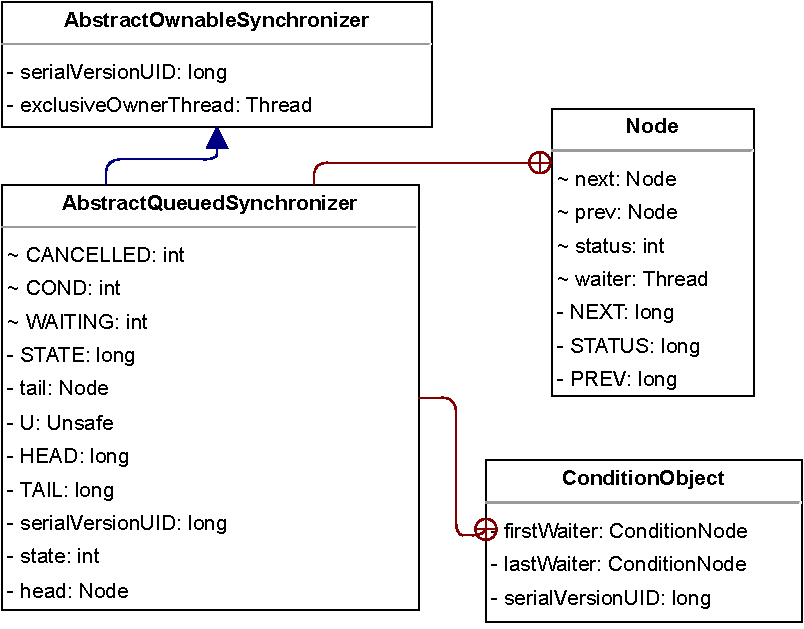
\includegraphics[width=0.6\linewidth]{../../../Images/AQS.pdf}
\end{center}

AQS 核心思想是,如果被请求的共享资源空闲,则将当前请求资源的线程设置为有效的工作线程,并且将共享资源设置为锁定状态。如果被请求的共享资源被占用,那么就需要一套线程阻塞等待以及被唤醒时锁分配的机制,这个机制 AQS 是用 CLH(虚拟的双向队列) 队列锁实现的,即将暂时获取不到锁的线程加入到队列中。

AQS 是一个 FIFO 双向队列,他有两个关键的内部类,他们的关键属性如下:
\begin{itemize}
    \item Node: 队列元素(没有公有方法)
    \begin{itemize}
        \item Thread waiter: 存放进入 AQS 队列的线程。Node 有两个子类用于标记线程阻塞原因:
        \begin{itemize}
            \item SharedNode: 标记线程是获取共享资源时被挂起进入 AQS 队列。
            \item ExclusiveNode: 标记线程时获取独占资源时被挂起后进入 AQS 队列。
        \end{itemize}
        \item int status: 用于记录当前线程等待状态,提供了三个常量:
        \begin{itemize}
            \item WAITING: 普通的等待状态。
            \item CANCELLED: 线程被取消。
            \item COND: 条件等待。
        \end{itemize}
    \end{itemize}
    \item ConditionObject: 条件变量,加强版 notify 和 wait 操作,下文细嗦。
    \begin{itemize}
        \item ConditionNode: 继承自 Node 的内部类,记录等待节点顺序。
        \item firstWaiter/lastWaiter: 用于记录第一和最后一个等待线程节点。
    \end{itemize}
\end{itemize}

AQS 最关键的属性是 state,不同的锁对其有不同的用法:
\begin{itemize}
    \item ReentrantLock: 表示当前线程获取锁的可重入次数。
    \item ReentrantReadWriteLock: 高于 16 表示读状态,低于16表示可重入次数。
    \item semaphore: 当前可用信号数。
    \item CountDownlatch: 计数器当前的值。
\end{itemize}

对于AQS来说,线程同步的关键是对状态值state进行操作。根据state是否属于一个线程,操作state的方式分为独占方式和共享方式。AQS 通过 acquire 系方法获取资源,release 系方法释放资源。共享和独占资源对应的方法不同:

\begin{itemize}
    \item 使用独占方式获取的资源是与具体线程绑定的,就是说如果一个线程获取到了资源,就会标记是这个线程获取到了,其他线程再尝试操作state获取资源时会发现当前该资源不是自己持有的,就会在获取失败后被阻塞。
    \item 对应共享方式的资源与具体线程是不相关的,当多个线程去请求资源时通过CAS方式竞争获取资源,当一个线程获取到了资源后,另外一个线程再次去获取时如果当前资源还能满足它的需要,则当前线程只需要使用CAS方式进行获取即可。
\end{itemize}

\subsubsection*{获取与释放资源}

在前面我们已经了解到,state 属性值的具体含义由子类赋予,因此与之相关的操作也全部由子类负责,父类仅提供接口。

在独占模式下,获取与释放资源有如下过程:

\begin{itemize}
    \item 获取资源: acquire(int arg) 方法。
\begin{Java}
public final void acquire(int arg) {
    if (!tryAcquire(arg))   // 具体实现由子类提供
        acquire(null, arg, false, false, false, 0L);
}
\end{Java}
    \begin{itemize}
        \item 首先会使用 tryAcquire(arg) 方法尝试获取资源,具体是设置状态变量 state 的值。
        \item 如果成功,直接返回。
        \item 如果失败,将当前线程封装为 ExclusiveNode 插入到 AQS 队列的尾部,调用 LockSupport.park 方法挂起自己。
    \end{itemize}
    \item 释放资源: release(int age) 方法。
\begin{Java}
public final boolean release(int arg) {
    if (tryRelease(arg)) {  // 同样由子类实现
        signalNext(head);   // 激活第一个被阻塞的线程并尝试获取资源
        return true;
    }
    return false;
}
\end{Java}
    \begin{itemize}
        \item 首先尝试使用tryRelease操作释放资源,具体也是操作 state 的值。
        \item 调用 LockSupport.unpark 激活 AQS 队列里被阻塞的第一个线程。
        \item 被激活的线程调用 acquire 方法,尝试获取资源。
    \end{itemize}
\end{itemize}

在共享模式下,获取与释放资源的操作类似,不过在获取资源失败后会线程会被封装为 SharedNode 插入队尾。

除了上述介绍的方法外,还需要重写 isHeldExclusively()方法,来判断锁是否已经被持有。

AQS 还提供了带 Interruptibly 后缀的 acquire 方法,不带Interruptibly关键字的方法的意思是不对中断进行响应,那么该线程不会因为被中断而抛出异常,而带Interruptibly关键字的方法要对中断进行响应。

虚拟的双向队列不存在队列实例,仅存在结点之间的关联关系,因此 AQS 每次入队操作实质上都是将线程封装成 Node 节点后添加进双向链表的操作。

\subsubsection{条件变量的支持}

正如 notify 和 wait 是配合 synchronized 内置锁实现线程间同步,ConditionObject(条件变量)的 signal 和 await 方法也是用来配合锁(AQS 实现的锁)实现线程同步的。不同点在于 synchronized 是共享线程独占锁,而 AQS 的锁可以对应多个条件变量。

\begin{Java}
public class ConditionObject implements Condition, java.io.Serializable
\end{Java}

在调用共享变量的notify和wait方法前必须先获取该共享变量的内置锁,同理,在调用条件变量的signal和await方法前也必须先获取条件变量对应的锁。

下面看一个 ReentrantLock(AQS 实现) 例子:

\begin{Java}
ReentrantLock lock = new ReentrantLock();   // 创建一个 ReentrantLock 锁
Condition condition = lock.newCondition();  // 创建一个条件变量

lock.lock();    // 获取锁
try {
    System.out.println("begin wait");
    condition.await();      // 阻塞挂起当前线程
    System.out.println("end wait");
} catch (Exception ex) {
    ex.printStackTrace();
} finally {
    lock.unlock();      // 释放锁
}
\end{Java}

这里的一些操作解释如下:
\begin{itemize}
    \item Lock 对象: 等价于 synchronized 加上共享变量。
    \item lock.lock(): 等价于进入 synchronized 块尝试获取锁。
    \item lock.unlock(): 等价于退出 synchronized 块释放锁。
    \item await() 方法: 等价于 Object 的 wait() 方法。
    \item signal() 方法: 等价于 Object 的 notify() 方法。
\end{itemize}

当线程调用条件变量的 await() 方法时(先调用 lock() 方法),在内部会构造一个 ConditionNode 型的 node 节点,然后插入节点,之后当前线程会释放获取的锁并被阻塞挂起。await() 方法的部分源码如下:

\begin{Java}
public final void await() throws InterruptedException {
    if (Thread.interrupted())
        throw new InterruptedException();
    // 创建新的节点
    ConditionNode node = new ConditionNode();
    // 释放当前线程获取的锁,插入节点
    int savedState = enableWait(node);
    // 阻塞挂起当前线程
    LockSupport.setCurrentBlocker(this);
    ......
}
\end{Java}

继续深入看一下如何获取锁并插入节点:

\begin{Java}
private int enableWait(ConditionNode node) {
    if (isHeldExclusively()) {  // 锁被持有
        node.waiter = Thread.currentThread();   // 将线程装入节点
        node.setStatusRelaxed(COND | WAITING);
        ConditionNode last = lastWaiter;
        if (last == null)
            firstWaiter = node;
        else
            last.nextWaiter = node;     
        lastWaiter = node;              // 插入节点完成,注意这是一个单向队列
        int savedState = getState();
        if (release(savedState))
            return savedState;
    }
    node.status = CANCELLED; // 获取锁失败
    throw new IllegalMonitorStateException();
}
\end{Java}

当多个线程同时调用lock.lock()方法获取锁时,只有一个线程获取到了锁,其他线程会被转换为Node节点插入到lock锁对应的AQS阻塞队列里面,并做自旋CAS尝试获取锁。

如果获取到锁的线程又调用了对应的条件变量的await()方法,则该线程会释放获取到的锁,并被转换为Node节点插入到条件变量对应的条件队列里面。

当另外一个线程调用条件变量的signal()或者signalAll()方法时,会把条件队列里面的一个或者全部Node节点移动到AQS的阻塞队列里面,等待时机获取锁。

一个锁对应一个 AQS 阻塞对象,对应多个条件变量。下图解释了条件队列与 AQS 阻塞队列的关系:

\begin{figure}[H]
    \centering
    \begin{tikzpicture}[scale = 1]
        \node[draw] (lock) at (0,0) {Lock}; 
        \foreach \y in {1,0,-1} {
            \node[draw] (Condition-\y) at (3,\y) {Condition};
            \node[draw] (条件队列-\y) at (6,\y) {条件队列};
            \draw[-Stealth] (Condition-\y) -- (条件队列-\y);
            \draw[-Stealth] (lock) -- (Condition-\y);
        }
        \node [draw,above,text width=1em] (AQS) at (-2,-2) {A Q S 阻塞队列};
        \draw [-Stealth] (lock) -- (AQS);
    \end{tikzpicture}
    \caption{条件队列}
    \label{fig:条件队列}
\end{figure}

\subsection{ReentrantLock 独占锁}

\subsubsection*{Lock 接口与 ReentrantLock 基础}

所有锁都需要实现 Lock 接口,它提供了最基础的方法:
\begin{itemize}
    \item void lock(): 获取锁。
    \item void lockInterruptibly(): 获取锁,被中断则抛异常。
    \item boolean tryLock(): 尝试获取锁,不会引起阻塞。
    \item boolean tryLock(long time, TimeUnit unit): 在一段时间内尝试获取锁。
    \item void unlock(): 释放锁。
    \item Condition newCondition(): 获取条件变量。
\end{itemize}

ReentrantLock 是可重入的独占锁,同时只能有一个线程可以获取该锁,其他获取该锁的线程会被阻塞而被放入该锁的AQS阻塞队列里面。

ReentrantLock 只有一个功能性成员变量: Sync sync,Sync 继承自 AQS 重写了一些方法。ReentrantLock 本质上还是使用 AQS 来实现的,可以根据参数决定它是一个公平锁还是非公平锁。

\begin{Java}
public ReentrantLock() {
    sync = new NonfairSync();
}

public ReentrantLock(boolean fair) {
    sync = fair ? new FairSync() : new NonfairSync();
}
\end{Java}

其中 NonfairSyn 和 FairSync 继承自 Sync,分别实现了锁的非公平与公平策略。

在这里,state 表示线程获取锁的可重入次数,默认情况下,state = 0 表示当前锁没有被任何线程持有。当一个线程第一次获取该锁时会尝试使用 CAS 设置 state 值为1,如果 CAS 成功则当前线程获取了该锁,然后记录该锁的持有者为当前线程。在该线程没有释放锁的情况下第二次获取该锁后,状态值被设置为2,这就是可重入次数。在该线程释放该锁时,会尝试使用CAS让状态值减1,如果减1后状态值为0,则当前线程释放该锁。

\subsubsection*{公平锁与非公平}

在 AQS 中,我们说过
















\newpage